\documentclass [10pt, a4paper, onecolumn, oneside] {scrreprt}
\usepackage[italian, english]{babel}
\usepackage[utf8]{inputenc}
\usepackage[T1]{fontenc}


%% Matematica
\usepackage{amsmath, amssymb}
\usepackage{xfrac}
\usepackage{units}
\usepackage{sansmath}


%%% PAGE DIMENSIONS
\usepackage{geometry} % to change the page dimensions
%\geometry{margins=2in} % for example, change the margins to 2 inches all round
%\geometry{landscape} % set up the page for landscape
% read geometry.pdf for detailed page layout information
%\usepackage{layaureo}
\usepackage{indentfirst}
%\usepackage{booklet}
\usepackage{lscape}


%% Note a fine capitolo
\usepackage{endnotes}
\numberwithin{endnote}{chapter}
\renewcommand{\theendnote}{(\roman{endnote})}
\renewcommand{\notesname}{Note}
\usepackage[stable]{footmisc}

%% Testatine
\usepackage{scrhack}
\pagestyle{headings}
%\usepackage[Lenny]{fncychap}

%% Biliografia
% citare usando `` \footnote{ \cite{cit:key}}}''
\usepackage{natbib}
%\usepackage[style=alphabetic]{biblatex}

%% Disegno
\usepackage{float}
\usepackage[center]{caption}
  \captionsetup{format=hang,labelfont={sf,bf},font=small}
\usepackage{subcaption}
\usepackage{sidecap}
\usepackage[siunitx]{circuitikz}
  \usetikzlibrary{decorations.pathmorphing,calc,3d, patterns}
  \usetikzlibrary{circuits}
\usepackage{pdfpages}
\usepackage{pgfplots}
  \pgfplotsset{/pgf/number format/use comma,compat=newest}
%\usepackage[pdftex]{graphicx}
\usepackage{qtree} % dendrogammi U_U

%% Codice
\usepackage{listings}
\addto\captionsitalian{%
\renewcommand{\lstlistingname}{Codice}}
\addto\captionsitalian{%
\renewcommand{\lstlistlistingname}{Elenco dei codici}}
\lstset{numbers=left, numberstyle=\tiny, stepnumber=1}

%% Faccine
\usepackage {MnSymbol, wasysym, marvosym}

%% Altri simboli
\usepackage{textcomp, wasysym}
\usepackage{cancel}
\usepackage{cases}% http://ctan.org/pkg/cases
\usepackage{framed}

%% Acronimi
\usepackage[smaller,printonlyused,withpage]{acronym}
 \acrodef{iic}[I$^2$C]{Inter-Integrated Circuit}
%  {\small Protocollo di comunicazione seriale \par}
 \acrodef{svm}[SVM]{Support Vector Machine}
%  {\small Macchina a vettori di supporto \par}
 \acrodef{spra}[SPRA]{Simple Pattern Recognition Algorithm}
 \acrodef{rbfk}[RBFK]{Radial Basis Function Kernel}
 
%% Sommario e abstract
\newenvironment{abstracts}
{\titlepage\vspace*{\fill}}
{\vspace*{\fill}\endtitlepage}
\renewenvironment{abstract}
{\vspace*{\fill}
\begin{center}\bfseries\abstractname\end{center}%
\quotation}
{\endquotation\vspace*{\fill}}

%% Togliere le scritte "capitolo" e altro 
\makeatletter	% NON commentare!
%\def\@makechapterhead#1{%
%  \vspace*{50\p@}%
%  {\parindent \z@ \raggedright \normalfont
%    \vskip 20\p@
%    \interlinepenalty\@M
%    \Huge \bfseries #1\par\nobreak
%    \vskip 40\p@
%  }}
\makeatother	% NON commentare!

%% Collegamenti ipertestuali
\usepackage{xcolor}
\usepackage{hyperref}
\hypersetup{
pdfauthor={Manuel Iurissevich},%
pdftitle={Valutazione gesti motori},%
pdfstartpage=5, pdfstartview=FitV,%
	colorlinks,
	linkcolor={red!0!black},
	citecolor={green!0!black},
	urlcolor={blue!0!black}
}

% EURO valuta
\usepackage{eurosym}

% dimensioni carattere
\usepackage{relsize}




\pagenumbering{roman}
\title{Sviluppo di un sistema per la valutazione di gesti motori}
\author{Manuel Iurissevich}
\date{} % delete this line to display the current date

%%%%%%%%%%%%%%%%%%%%%%%%%%%%%%%%%%%%%%%%%%%%%%%%%%%%%%%%%
%%% BEGIN DOCUMENT %%%%%%%%%%%%%%%%%%%%%%%%%%%%%%%%%%%%%%
\begin{document}
%%%%%%%%%%%%%%%%%%%%%%%%%%%%%%%%%%%%%%%%%%%%%%%%%%%%%%%%%
%\maketitle

\includepdf{Capitoli/0/Frontespizio}



\newcommand{\iic}{{\relsize{-1} I$^2$C}}
\newcommand{\usb}{{\relsize{-1} {USB}}}
\newcommand{\sda}{{\relsize{-1} {SDA}}}
\newcommand{\scl}{{\relsize{-1} {SCL}}}
\newcommand{\vcc}{{\relsize{-1} \(V_{CC}\)}}
\newcommand{\master}{\textit{master}}
\newcommand{\slave}{\textit{slave}}
\newcommand{\Ack}{\textit{acknowledge}}
\newcommand{\ack}{\relsize{-1}{ACK}}
\newcommand{\pullup}{\textit{pull-up}}








\begin{abstracts}
	\selectlanguage{italian}
		\begin{abstract}
	Italiano
		\end{abstract}

	\selectlanguage{english}
		\begin{abstract}
	Inglese
		\end{abstract}
	\selectlanguage{italian}
\end{abstracts}

%\vfill
% \begin{center} {\bfseries Istruzioni per la versione elettronica} \end{center}
\paragraph{}
	Il documento \`e un ipertesto e contiene pertanto dei collegamenti cliccabili.
	Sono cliccabili le voci dell'indice,
	i rimandi alle note a pi\`e di pagina,
	le citazioni dei riferimenti bibliografici,
	gli elenchi di figure, tavole e codici.
	Il programma di lettura dovrebbe fornire un pulsante \textsf{Indietro},
	con cui ritornare rapidamente al punto di testo in cui si leggeva
	prima di cliccare sul collegamento.
	
	La quasi totalit\`a delle immagini sono create o importate in un formato vettoriale
	che permette di ingrandirle pi\`u die dieci volte.
	
	La numerazione delle pagine inizia dal primo capitolo.
	Le precedenti sono numerate in romano minuscolo
	da `i' (la pagina del titolo) a `v' (quella dell'indice).
	La funzione \textsf{Vai alla pagina} dovrebbe
	riconoscere correttamente questa numerazione
	ma alcuni software (anche le stampanti!) potrebbero iniziare 
	a numerare le pagine direttamente dal titolo.
																\vspace{1in}
\begin{center} {\bfseries Instructions for the electronic version} \end{center}
\paragraph{}	\selectlanguage{english}
	Table of contents, footnotes, references,
	lists of figures, tables and codes have clickable links.
	The text reader should provide a \textsf{Back} button. 
	Images are more than ten times zoomable.
	
	Pages are numbered lowercase roman in the front matter
	from `i' (title page) to `v' (table of contents).
	Function \textsf{Go to page} should correctly work with these pages too,
	but some readers (and print utilities!) could start arabic numbering from title page
	without resetting at the first chapter.\vfill



\selectlanguage{italian}

	
\setcounter{tocdepth}{2}
\tableofcontents
\vfill
\thispagestyle{empty}
\eject

\pagenumbering{arabic}
%\pagestyle{useheadings}

\newpage
\thispagestyle{empty}
\mbox{}





\chapter{Introduzione} \label{cap:intro}
		{\bfseries
\vspace{1in}

\paragraph{}
Sarà per prima cosa fornita una definizione dell'oggetto del lavoro,
cioè il {\rm gesto motorio}, per poi proseguire con l'esposizione del problema generale
a cui si cerca di dare una possibile soluzione.


\paragraph{}
Si discuteranno le principali soluzioni fornite dalla letteratura
e si farà accenno alle più recenti e pertinenti.

\paragraph{}
Seguiranno obiettivi, vincoli e risorse del progetto.

\paragraph{}
Il capitolo termina con una breve introduzione alla biomeccanica.

\vfill
} \vfill\eject
	\section{Definizione} \label{sez:defnizione}
		Nei prossimi paragrafi si dà al lavoro un inquadramento generale.


%% Definizione
	\subsection{Il gesto motorio} \label{ssez:definizione}

\begin{quotation}
	``\textbf{Il movimento} è il risultato dell'attivazione
	di un limitato distretto muscolare che produce lo spostamento nello spazio
	di una o più articolazioni.
	Esempi: \emph{flessione di un dito}, rotazione di un polso.
	\textbf{L'atto motorio} è il \emph{risultato di più movimenti},
	eseguiti sinergicamente e in maniera fluida, che coinvolgono più articolazioni.'' 
%	-- Mandolesi L.(2012), \emph{Neuroscienze dell'attività motoria.} Springer, Milano
\cite{cit:mandolesi}
\end{quotation} 

\begin{quotation}
	``\textbf{Il gesto motorio} raffigura la comunicazione non verbale
	mediante l'atto visibile relativo all'esecuzione,
	più o meno abile, di una risposta motoria.
	La somma di più gesti motori in successione è denominata \textbf{atto motorio}.''
%	-- Lestini G., \emph{Il significato di psicomotricità.} http://motricitascuola.altervista.org/
\cite{cit:lestini}
\end{quotation}

La definizione è ambigua.
Vista l'astrattezza del termine \emph{gesto},
si è preferito nel titolo del lavoro specificare che si tratterà di gesti \emph{motor\^i}.
Il sinonimo \emph{movimento},
troppo generico per essere inserito nel titolo di una tesi in ingegneria,
sarà invece utilizzato nel testo
una volta stabiliti gli ambiti di studio: elettronica, neuroscienze, biomeccanica.





% Problema
	\subsection{Il problema}

Il problema fondamentale al quale si cerca di dare una soluzione
è utilizzare tecniche non invasive per fornire dati quantitativi sui movimenti
a medici e pazienti (come ad allenatori ed atleti),
che possano essere loro di aiuto a migliorare la qualità degli esercizi
(sportivi o fisioterapici)
e a prevenire infortuni.

Particolare attenzione va posta al problema dell'\emph{autonomia} dei soggetti.
Se esercitarsi porta benefici, farlo in modo errato può provocare danni alla parsona.
D'altro canto non è possibile per un esperto garantire assistenza costante,
per fornire indicazioni e correzioni, per lo meno per questioni di costo.

È per questo che ci si sforza di fornire soluzioni per il supporto domestico ai pazienti,
come anche software per la ginnastica fai-da-te.




% Stato dell'arte
	\subsection{Lo stato dell'arte}
Le soluzioni proposte per questo genere di problemi
sono solitamente basate su tecniche di visione artificiale.
Queste richiedono però l'installazione di telecamere
e una luce appropriata alle riprese,
necessità che vincolano i movimenti all'interno di una stanza.
Sono soluzioni valide in un laboratorio medico o in una palestra,
meno valide in ambiente domestico,
quasi improponibili in un campo sportivo o in un parco.



Tra le soluzioni basate sugli accelerometri
le più pertinenti da citare in questo testo
sono un guanto proposto per migliorare la tecnica
nel lancio dei dardi \footnote{\,\cite{cit:guanto}}
e una manica per prevenire gli infortuni nel baseball \footnote{\cite{cit:manica}}.





 \vfill
	\section{Specifiche} \label{sez:specifiche}
		%%%%%%%%%%%%%%%%%%%%%%%%%%%%%%%%%%%
%\vspace{12pt}
%\vspace{0.25in} \hrule \vspace{0.1in}

Grazie al colloquio con un esperta e a uno studio preliminare
si possono definire le caratteristiche specifiche del progetto. 

\subsection{Colloquio con l'esperta}
Durante un colloquio con un'esperta in materia
si è scelto di studiare il \textbf{Port de Bras},
movimento fondamentale della \emph{danza classica}.
Il gesto è stato scelto,
oltre che per le sue caratteristiche cinematiche,
perché permette di concentrare lo studio su un solo arto
pur senza perdere generalità nella soluzione.

In questa fase, l'esperta ha definito il protocollo di esecuzione
del gesto corretto e i principali errori.
Per approfondimenti, vedere la \textsc{Sottosezione~\ref{ssez:descrizionedelmovimento}}.




\subsection{Obiettivi}
Una volta che il \emph{gesto corretto} è definito,
si può cercare una soluzione al problema specifico di questo lavoro.

Si vuole un sistema
costituito da un dispositivo facilmente maneggiabile
e da un programma di calcolo,
che valuti il movimento eseguito
come lo valuterebbe un esperto.

Si realizzerà un \emph{classificatore binario},
capace di rispondere con $vero$ o $falso$
alla domanda:
\begin{quote}
Il movimento appena eseguito \emph{appartiene} all'insieme dei gesti corretti?
\end{quote}.




\subsection{Vincoli}
La soluzione è vincolata dall'utilizzo di un basso numero di sensori
e dalla semplicità di definizione delle regole.




\subsection{Risorse}

Le risorse a disposizione sono accelerometri triassiali per l'acquisizione,
tecniche di apprendimento automatico per la classificazione,
il programma di calcolo MatLab per l'elaborazione numerica dei dati
e il microcontrollore Arduino per l'interfaccia trai sensori e il calcolatore.
 \vfill
	\section {La biomeccanica}
	  \label{sez:biomeccanica}
		Si ritiene opportuno introdurre qualcuno dei concetti fondamentali della biomeccanica,
per meglio comprendere le scelte fatte in fase di progettazione
\footnote{\cite{donskoi}}.

\begin{quote}
 {L'oggetto} della biomeccanica sono le azioni motorie dell'Uomo come sistema
di movimenti mutuamente coerenti e posture del corpo.
\end{quote}

\begin{quote}
 {Il metodo} della biomeccanica \`e basato su un'analisi e una sistesi sistematica
del movimento sulla base di caratteristiche quantitative,
soprattutto la modellazione matematico-cibernetica del movimento.
\end{quote}


\begin{quote}
I muscoli di norma non funzionano isolati bens\`i a gruppi.
Le interazioni avvengono all'interno dei gruppi muscolari e anche tra gruppi.
\end{quote}
Quindi può non essere necessario monitorare ogni muscolo
o segmento della catena cinematica per valutare il movimento.

\begin{quote}
La quantit\`a di gradi di libert\`a corrisponde al numero dei possibili movimenti
angolari e lineari indipendenti di un corpo
\textit {Si dice \emph {libero} un corpo che non sia costretto nei propri movimenti.}
Tale corpo pu\`o spostarsi in tre dimensioni e ruotare su tre assi
e ha quindi sei gradi di libert\`a.
Fissando uno, due, tre punti si riducono i gradi di libert\`a a tre, uno, zero.
\end{quote}


\begin{quote}
La quantit\`a di assi principali di un'articolazione corrisponde
alla quantit\`a di gradi di libert\`a di un arto rispetto ad un altro.
Il piano di movimento \`e perpendicolare all'asse di rotazione
e caratterizza l'orientamento e lo spostamento di un arto.
L'ampiezza del movimento rappresenta lo spostamento angolare
di un arto da una posizione limite a un'altra.
\end{quote} \vfill
% \theendnotes



\chapter{Acquisizione} \label{cap:acquis}
		{\bfseries
\vspace{1in}

\paragraph{}
Il capitolo riguarda i componenti del sistema
dall'arto umano
all'ingresso del calcolatore. 
\\

Si tratter\`a quindi il posizionamento dei sensori sull'arto
e si far\`a una breve digressione sulla biomeccanica in generale,
per poi applicarla al sistema in questione.
\\

Per la parte elettrica, si confronteranno degli accelerometri
in commercio, tra quelli che rispettano le specifiche poste.
\\

Infine la trasmissione del segnale, con un'introduzione al protocollo \iic{} e la conversione in \usb{}.

\vfill
} \vfill\eject
	\section{Meccanica} \label{sez:meccanica}
		Occorre studiare la catena cinematica coinvolta nel movimento
per individuare i punti in cui fissare i sensori
e le caratteristiche che possono portare a una classificazione migliore.

Si propone quindi il modello della semplice catena \emph{gomito-polso}
e alcune considerazione sul numero e la disposizione degli accelerometri,
a seconda dell'applicazione.

\subsection{Studio della catena cinematica}
\label{ssez:cat_cine}

Durante le prime fasi della progettazione
si è studiata la cinematica del movimento più semplice
su cui sono stati provati i vari metodi di classificazione.

Per questi è abbastanza semplice definire le regole di valutazione,
tanto che potrebbero essere inserite direttamente nel sistema.


Il movimento proposto è il \emph{sollevamento del bicipite}.
I sollevamenti sono effettuati a gomito vincolato,
quindi soltanto con l'avambraccio.
Durante i movimenti ``giusti'' la traiettoria \`e mantenuta
il pi\`u possibile dritta, mentre durante quelli ``sbagliati''
si devia dall'asse verticale.

Il sensore \`e tenuto in mano in maniera
con l'asse $z$ uscente dal palmo.
Il polso \`e rigido.

\begin{figure}
  \centering
	\begin{tikzpicture}[%
molla/.style={decorate,decoration={snake,post length=5,amplitude=5,pre length=5,segment length=5}, thick},
thick%
]
\sffamily \sansmath
%	\draw [help lines] (0, 0) grid (8, 5);
	
	\draw (8, 0) -- (0, 0);
	
	\draw (0, 3) circle (0.3)
		node at (0, 3) {$\bullet$};
	\node [] at (-.8, 3) {spalla};
	\draw (0, 3) -- (4, 0);
	\draw (4, 0) circle (0.3)
		node {$\bullet$};
	\node [] at (4, 0.8) {gomito};
	\draw (4, 0) -- (7, 2);
	\draw (7, 2) circle (0.3)
		node {$\bullet$};
	\draw (7, 2) -- (8, 3)
		node [pos=0.5, right] {mano};
	\draw (7.2, 2.4) -- (7.9, 3.1)
		node [pos=0.5, left] {cell};

  \end{tikzpicture}
  \caption{Schema approssimativo.}
  \label{fig:gomito2}
\end{figure}

Fissata che sia la posizione della punta del gomito,
l'avambraccio ha tre gradi di libert\`a di rotazione.
Il polso pu\`o ruotare in altri due modi,
per un totale di cinque gradi di libert\`a.

In questa dimostrazione si cerca di sopprimere
i movimenti del polso e la rotazione sull'asse dell'avambraccio.
Fatto questo, si considera corretta l'esecuzione del movimento
quando non c'\`e variazione dell'angolo longitudinale
ma solo di quello latitudinale (vedi \textsc{Figura \ref{fig:gomito1}}).

Utilizzando i formalismi della robotica
%\footnote{ \cite{deluca}}
si pu\`o scrivere la \textsc{Tabella \ref{tab:robo}}.
Il sistema di riferimento $S_{3}$ \`e quello del sensore.

Secondo questa notazione:
\begin{itemize}
	\item [$\theta_{1}$] {$\in [0, \pi/2]$ \`e l'unico parametro che si vuole variare}
	\item [$\theta_{2}$] {$\in [-\pi/2, \pi/2]$ dovrebbe rimanere fisso, meglio se nullo}
	\item [$\alpha_{1}:$] la rotazione attorno a $y_{1}$ \`e il principale errore da individuare
	\item [--] {altri parametri si considerano nulli o costanti}
\end{itemize}

\begin{figure}
  \centering
    \begin{tikzpicture}[%
molla/.style={decorate,decoration={snake,post length=5,amplitude=5,pre length=5,segment length=5}, thick},
thick%
]
\sffamily \sansmath
%	\draw [help lines] (0, 0) grid (8, 8);
	
	\draw (0:0) -- (0:5);
	
%	\draw (0, 3) circle (0.3)
%		node {$\bullet$};
%	\draw (0, 3) -- (4, 0);
	\draw (0, 0) circle (0.3)
		node {$\bullet$};
	\draw (30:5) circle (0.3)
		node {$\bullet$};
		
	\draw (0, 0) -- (30:5);
	\draw (30:5) -- ++(45:2);
	\draw (4.5, 3) -- ++(45:1.5);

	\node [] at (25:5.3) {P};
	\node [] at (-0.5, 0) {G};
	\node [] at (5.0, 4) {C};

	\draw [->, dotted, thin] (0:5) -- (0:8)
		node [pos=1, above] {$x_{0}$};
	\draw [->, dotted, thin] (90:0) -- ++(90:3)
		node [pos=1, left] {$y_{0}$};

	\draw [->, dotted, thin] (30:5) -- ++(30:3)
		node [pos=1, above] {$x_{1}$};
	\draw [->, dotted, thin] (0:0) -- (30+90:3)
		node [pos=1, left] {$y_{1}$};

	\draw [->, dotted, thin] (30:5) -- ++(45:5)
		node [pos=1, above] {$x_{2}$};
	\draw [->, dotted, thin] (30:5) -- ++(45+90:3)
		node [pos=1, left] {$y_{2}$};

	\draw [->, dotted, thin] (4.5, 3) -- ++(45:3)
		node [pos=1, above] {$y_{3}$};
	\draw [->, dotted, thin] (5.0, 3.5) -- ++(45+90:3)
		node [pos=1, left] {$z_{3}$};

  \end{tikzpicture}
 
  \caption{Sistemi di riferimento.}
  \label{fig:gomito1}
\end{figure}

\begin{table}
\centering
\caption{Parametri della catena cinematica}
\label{tab:robo}
\begin{tabular} {l c c c c}
	\hline
	$i$ & $\alpha_{i}$ & $a_{i}$ & $d_{i}$ & $\theta_{i}$\\
	\hline
	1 & 0 & 0 & 0 & $\theta_{1}$ \\
	2 & 0 & $\bar{GP}$ & 0 & $\theta_{2}$ \\
	3 & $\pi/2$ & $\bar{PC}$ & 0 & $\pi/2$ \\
	\hline
\end{tabular}
\end{table}





\subsection{Fissaggio del sensore all'arto}
\label{ssez:fissaggio}

Il punto più importante dove fissare i sensori è sicuramente al termine della catena,
cioè all'altezza del polso o del dorso della mano.
Qualora si necessitasse di più punti di osservazione,
si potrebbero fissare ulteriori sensori all'altezza del gomito e della spalla.
Si preferisce comunque ridurre il numero di sensori al minimo,
possibilmente a uno (sul polso).

Sebbene sia teoricamente possibile spostare il gomito
tenendo fermi polso e spalla (fermi rispetto a un sistema fisso),
un movimento del genere risulta quantomeno innaturale
ed è inverosimile che sia di qualche utilità.
Ai fini della valutazione della correttezza del gesto
si assume quindi che un errore commesso a livello della spalla
o del gomito si propaghi lungo la catena
potendo quindi essere rilavato da un sensore a valle.

Questa assunzione è importante nel caso si preferisca
un sistema basato sugli accelerometri contenuti negli \textit{smartphone},
spostando sul software il carico computazionale
e il bisogno di robustezza.
Diverso sarà il discorso quando si vorrà correggere il gesto
e non basterà sapere \emph{se} è stato commesso un errore
ma occorrerà sapere almeno \emph{dove e quando}.
 \vfill
	\section{Elettronica} \label{sez:elettronica}
		Seguendo il percorso del segnale elettrico dai sensori al calcolatore,
si motivano le scelte di progetto e
se ne espongono i principali aspetti.

\subsection{Sensori}
\label{ssez:sensori}

Descrizione di quelli utilizzati e confronto con gli altri.

  \subsection{Gli accelerometri} \label{ssez:accelerometri}
    Specifiche richieste (in ordine di priorità):
	\begin{itemize}
      \item [] {Uscita digitale}
	  \item [] {Accelerazione massima $\ge \pm8g$}
      \item [] {Frequenza di campionamento $\geq 100Hz$}
      \item [] {Digitalizzazione a profondità $\ge 8bit$}
      \item [] {Almeno due indirizzi disponibili}
      \item [] {Prezzo $\le$ 20\euro}
	\end{itemize}

    La \textsc{Tabella~\ref{tab:accelerometri}} mostra sinteticamente un confronto
    tra i sensori disponibili sul mercato.

	\begin{table}
		% Center the table
		\begin{center}
		% Title of the table
		\caption{Confronto tra gli accelerometri da acquistare}
		\label{tab:accelerometri}
		% Table itself: here we have two columns which are centered and have lines to the left, right and in the middle: |c|c|
		\begin{tabular}{r c c c c}
			% To create a horizontal line, type \hline
%			\hline
			% To end a column type &
			% For a linebreak type \\
Disp.  & Range ($\pm$g) & Codifica (bit) & Prezzo (\euro) & Interfaccia \\
			\hline
InvSen & 2-16           & 16         & 18,00          & \iic \\
mCube  & 2-16           & 8-14       & 11,32          &\iic, {\relsize{-1} SPI} \\
\textbf{AdaF} & \textbf{2-8} & \textbf{14} & \textbf{9,31} & \textbf{\iic} \\
SF MMA & 2-8            & 8, 12      & 10,03          & \iic \\
\textbf{ADXL345} & \textbf{2-16} & \textbf{10-13} & - & \textbf{\iic,{\relsize{-1} SPI}} \\
			\hline
		\end{tabular}
		\end{center}
	\end{table}
    
    \subsubsection {L'uscita digitale} \label{sssez:digitale}	
    Con l'uscita digitale, per ogni numero di accelerometri
    è sufficiente un unico \textit{bus} da tre cavi
	\footnote{\,Dipende da quanti indirizzi sono disponibili
	(vedi: \textsc{\ref{sssez:indirizzi}})}:
	dati, clock e massa;
    con l'uscita analogica è
\[
	cavi = accelerometri \times assi
\]
    quindi per quattro accelerometri triassiali occorrono
    \(4 \times 3  = 12\) cavi.
    A tanti cavi corrisponderebbero tanti ingressi analogici di microcontrollore.
    

    \subsubsection {Ampiezza e frequenza di campionamento} \label{sssez:accmax}
    Per determinare quale fosse l'ampiezza minima necessaria,
    sono stati usati due accelerometri già disponibili:
    il primo è all'interno di un telefono cellulare {\relsize{-1} GT-S7501};
    il secondo fa parte di un sistema di acquisizione professionale.
    Un sintetico confronto in {\relsize{-.5} \textsc{Tabella~\ref{tab:accelerometricasa}}}.
    Entrambi sono stati sottoposti a movimenti semplici e
    al lancio di un dardo.
	\begin{table}
		% Center the table
	  \begin{center}
		% Title of the table
		\caption{Confronto tra gli accelerometri già disponibili}
		\label{tab:accelerometricasa}
		% Table itself: here we have two columns which are centered and have lines to the left, right and in the middle: |c|c|
		\begin{tabular}{r c c}
			% To create a horizontal line, type \hline
%			\hline
			% To end a column type &
			% For a linebreak type \\
Disp.   & Range ($\pm$g) & Freq. Camp. (Hz)\\
			\hline
GT-S750 & 2              & 50 \\
Pro     & $>$30          & 10k \\
			\hline
		\end{tabular}
	  \end{center}
	\end{table}

    L'accelerometro di fascia bassa risponde adeguatamente a sollecitazioni deboli,
    mentre risulta totalmente inadeguato all'applicazione finale,
    sia per ampiezza che per frequenza di campionamento.
    Prima di ricorrere all'accelerometro professionale,
    si è cercato di ricostruire il segnale corrotto dalla saturazione.
    In \textsc{Figura~\ref{fig:ricostruzione}}
    il segnale da ricostruire è rappresentato in blu e
    in rosso il segnale corretto, mentre
    con il bollino nero si evidenzia l'ampiezza massima stimata.
    A posteriori, si vedrà che il segnale vero è più ampio.
    Si nota presto che la frequenza di campionamento
    dev'essere almeno raddoppiata.

%	\textbf{Cercare di standardizzare il grafico in b/n,
%		con i bollini e la legenda, e soprattutto in {\relsize{-.5} EPS}}.

% This is how you include a eps figure in your document. LaTeX only accepts EPS or TIFF files.
	\begin{figure}
		% Center the figure.
		\begin{center}
		% Include the eps file, scale it such that it's width equals the column width. You can also put width=8cm for example...
		\resizebox{\columnwidth}{!}{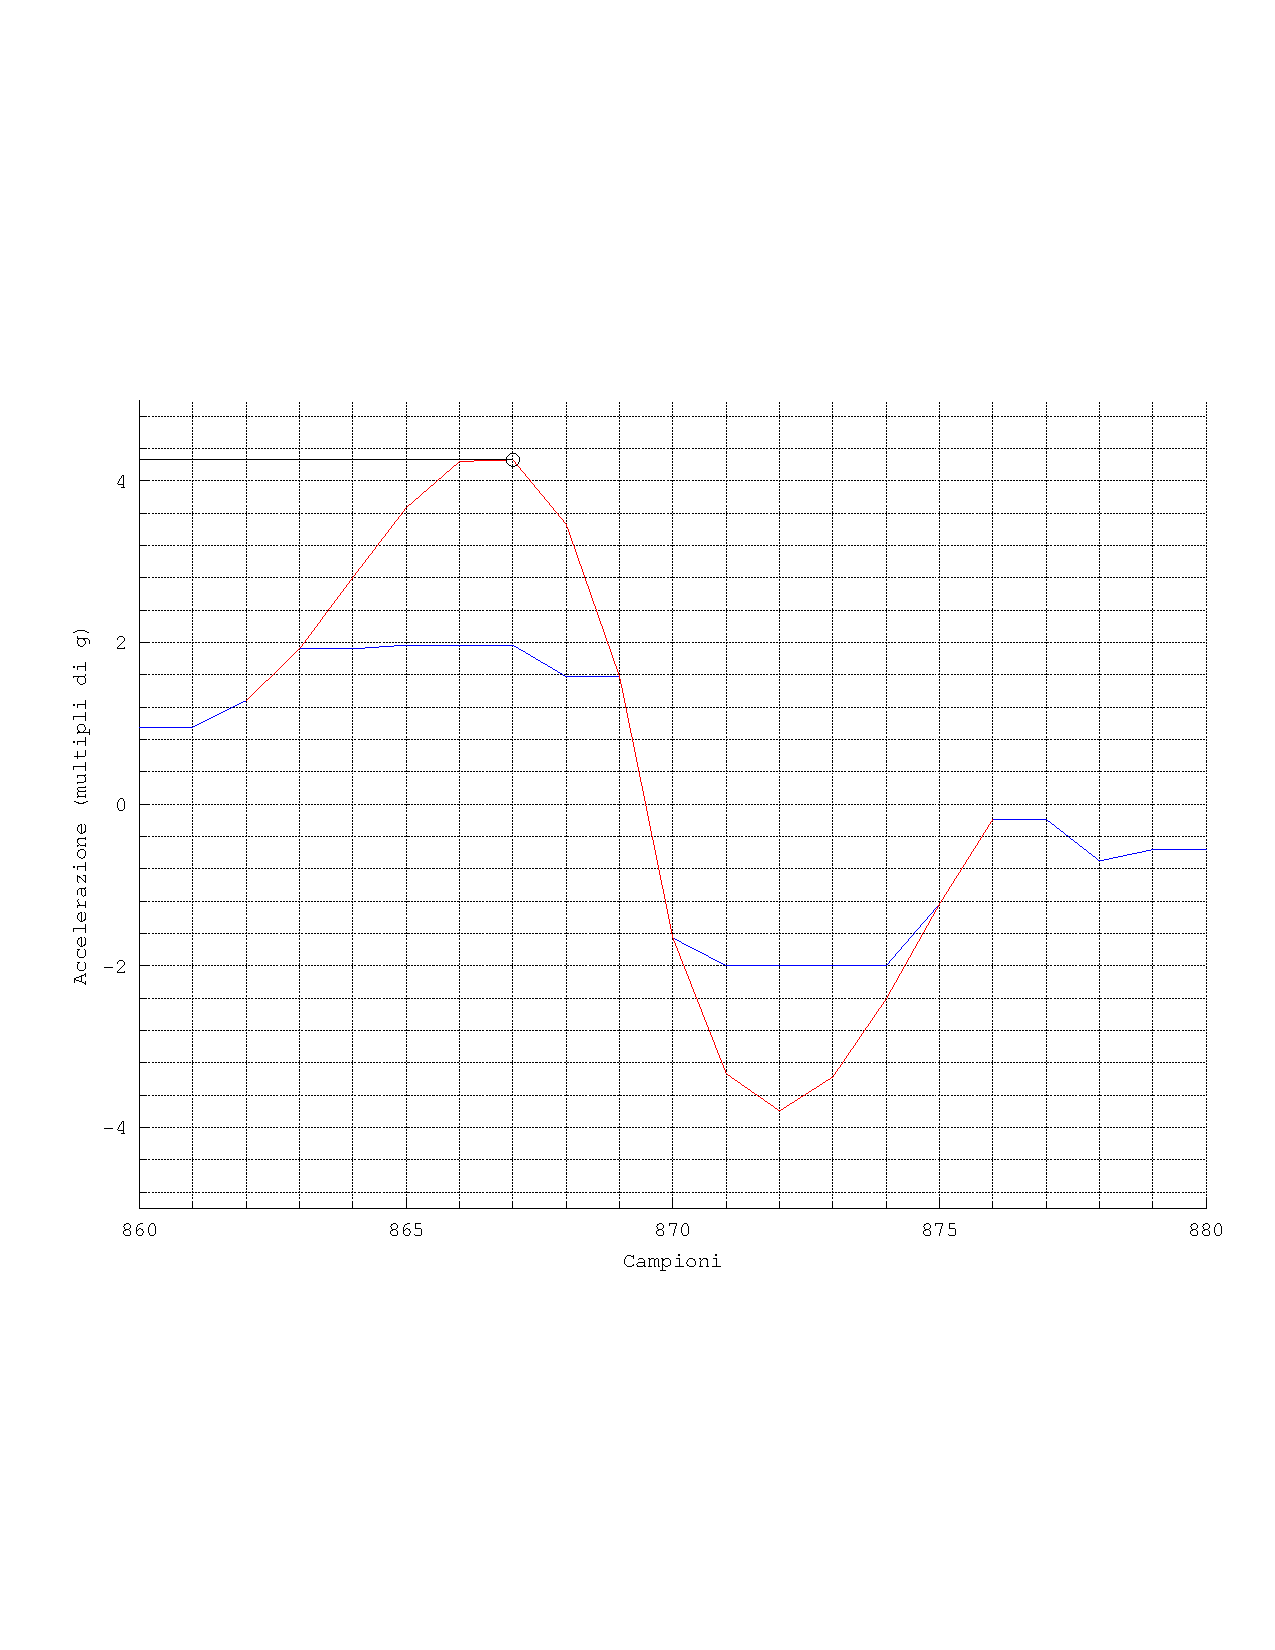
\includegraphics{taybella_copia.pdf}}
		% Create a subtitle for the figure.
		\caption{Esempio di ricostruzione di un segnale saturato}
		% Define the label of the figure. It's good to use 'fig:title', so you know that the label belongs to a figure.
		\label{fig:ricostruzione}
		\end{center}
	\end{figure}

	Con l'accelerometro di fascia alta si è invece potuto acquisire
    il vero movimento; da questo si sono ricavate le specifiche
    sugli accelerometri.
    
    
	\subsubsection {Indirizzi} \label{sssez:indirizzi}
    Come sarà spiegato in maggior dettaglio nella \textsc{Sezione~\ref{sez:protocollo_i2c}}
    il protocollo {\iic} richiede che in un determinato istante
    un dispositivo faccia da {\master} e gli altri da {\slave}.
    
    Concettualmente il calcolatore è {\master}
    \footnote{\,Il calcolatore non comunica direttamente sul \textit{bus} {\iic},
    quindi il vero {\master} è il processore del convertitore}
    e gli accelerometri sono {\slave}.
    All'inizio di ogni nuova comunicazione il \master{}
    scrive sul \textit{bus} l'indirizzo dello \textit{slave} interrogato.
    Il messaggio è lungo un byte ed è formato da 7 bit di indirizzo
    seguiti dal bit di comando: \texttt{1}\,=\,lettura e \texttt{0}=scrittura.
    
Il protocollo \iic{} mette quindi a disposizione
    \(2^7=128\) indirizzi \footnote{\,Sedici indirizzi sono riservati}
    ma i costruttori delle schede di sviluppo su cui sono montati gli accelerometri
    fissano tutti o quasi i piedini, lasciando disponibili uno o due indirizzi.
    Si rende quindi necessario l'utilizzo di linee separate o di un \textit{multiplexer}: avendo disponibile in casa un adattatore con due canali,
    si è scelto di percorrere la prima via.








\subsection{Trasmissione}
\label{ssez:trasmissione}

\section{Il protocollo I2C} \label{sez:protocollo_i2c}
{Nota: Tutta questa sezione fa riferimento alla guida~\footnote{\cite{cit:primer}}.}

\relsize{0}
%	Descrizione del protocollo con le solite figure.
    Fu progettato dalla Philips Semiconduttori (ora NXP) nel 1982
    per la comunicazione tra componenti sulla stessa scheda circuitale.
    La velocità standard è di 100kbit/s,
    accelerata a 400kbit/s (modalità veloce)
    oppure a 3,4Mb/s (alta velocità).
    A livello fisico le linee \sda{} e \scl{} sono a \emph{collettore aperto}
    (\textit{open-drain}),
    cioè possono essere forzate basse oppure \emph{lasciate} alte~\footnote{\cite{cit:primer}}.
	
\begin{figure}[t]
	\centering
\resizebox{\textwidth}{!}{
\includegraphics{I2C_data_transfer.png}}
    \caption{Diagramma temporale di una comunicazione \iic{}. S - Start; P - Stop; B - trasferimento di un bit; commutazione sul fronte di discesa del clock (blu). Opera di pubblico dominio di Marcin Floryan.}
    \label{fig:i2c_trans}
\end{figure}


    Pregi:
\begin{itemize}
	\item {sono necessarie soltanto due linee}
	\item {relazione {\master}-{\slave}, ciascuno con un indirizzo univoco}
	\item {il master genera il clock}
	\item {
    	possibilità di \textit{multimaster} tramite arbitraggio
   		\footnote {
        	non essendo utilizzato nel progetto,
        	questo aspetto non sarà trattato
        }
	}
\end{itemize}

\subsection{Considerazioni hardware}

\subsubsection{Configurazione tipica}
La \textsc{Figura \ref{fig:i2c_tipica}}
mostra la tipica configurazione di una linea {\iic}
con le resistenze $R_S$ in serie,
le resistenze $R_P$ di \pullup,
le capacità parassite $C_P$
e quella di \textit{crosstalk} $C_C$, di interferenza tra le linee.

Ciascun dispositivo può \footnote{\,dovrebbe poter}
intervenire soltanto abbassando la linea.

Le resistenze di {\pullup} possono essere inserite alla fine della linea
e per questo sono chiamate anche \textit{{\iic} termination};
hanno comunemente un valore di $1k\Omega$.

Le resistenze in serie possono essere molto basse o quasi nulle
a meno che non si abbia l'esigenza di proteggere il circuito da correnti esterne.
Per ogni dispositivo si considerano uguali le resistenze su {\sda} e {\scl}
\begin{equation}
	R_{S\,1,\,j}\,=\,R_{S\,2,\,j}\qquad \forall i.
\label{eqn:rs}
\end{equation}
Quando una linea è abbassata al livello logico \textsc{0},
la tensione è data dal partitore tra $R_P$ e $R_S$.
Per la linea $i$ comandata dal dispositivo $j$ è
\begin{align}
	V_{i}\,&=\,\frac{R_{S\,i,\,j}}{R_{S\,i,\,j}+R_{P\,i}}\;V_{CC} \\
    & =\,\frac{50}{50+1k}\;3.3V \,=\,157mV
\label{eqn:partitore}
\end{align}
La conseguenza positiva è che assegnando a ogni dispositivo un valore di $R_S$ differente,
è possibile per il progettista capire quale dispositivo sta agendo sulla linea.
Per contro, può accadere che questa tensione non sia abbastanza bassa da essere letta come \textsc{0} logico,
con le implicazioni descritte più avanti nel testo.

\begin{figure}
  \centering
  \resizebox{.9\linewidth}{!}{	\begin{tikzpicture}
\relsize{-1}
\node (nSDA1) at (-3,1) {};
\node (nSCL1) at (-3,-1) {};
\node (nSDA2) at (3,1) {};
\node (nSCL2) at (3,-1) {};
\node (nCondens1) at (0,1) {};
\node (nCondens2) at (0,-1) {};
\node (nPullUp1) at (-1,1) {};
\node (nPullUp2) at (1,-1) {};
\node (nFinto1) at (1,1) {};
\node (nFinto2) at (-1,-1) {};
\node (nAlimPullUp1) at (-1, 3) {};
\node (nAlimPullUp2) at (1, 3) {};
\node (nAlim1) at (-3, 3) {};
\node (nAlim2) at (3, 3) {};
\node (nMassaCap1) at (-1, -3) {};
\node (nMassaCap2) at (1, -3) {};
\node (nMassa1) at (-3, -3) {};
\node (nMassa2) at (3, -3) {};
\node (nSDAin1) at (-6, 1) {};
\node (nSDAout1) at (-6, 0) {};
\node (nSCLin1) at (-6, -1) {};
\node (nSCLout1) at (-6, -2) {};
\node (nSDAin2) at (6, 1) {};
\node (nSDAout2) at (6, 0) {};
\node (nSCLin2) at (6, -1) {};
\node (nSCLout2) at (6, -2) {};

%	
%	Resistenze in serie
\draw (nSDA1) to [resistor, l^=$R_{S11}$, o-, n=r11] (nPullUp1)
      (nSCL1) to [resistor, l^=$R_{S21}$, o-, n=r21] (nFinto2)
      (nFinto1) to [resistor, l^=$R_{S12}$, -o, n=r12] (nSDA2)
      (nPullUp2) to [resistor, l^=$R_{S22}$, -o, n=r22] (nSCL2);
%	
%	Resistori in parallelo
\draw (nAlimPullUp1) to [resistor, l^=$R_{P1}$, n=rp1] (nPullUp1)
      (nAlimPullUp2) to [resistor, l^=$R_{P2}$, n=rp1] (nFinto1);
%	
%	Condensatori
\draw (nCondens1) to [capacitor, *-*, n=cc] (nCondens2) 
      (nFinto1) to [short] (nPullUp2) to [capacitor, l^=$C_{P2}$, n=cp2] (nMassaCap2)
      (nPullUp1) to [short] (nFinto2) to [capacitor, l^=$C_{P1}$, n=cp2] (nMassaCap1);
\node at (.5,-.5) {$C_C$};
%	
%	Transistori
\draw (-3.5,-1) to [Tnmos=11, n=mos11] ++(0, 2)
	  (-4,-3) to [Tnmos=21, n=mos21] ++(0, 2);
\draw (3.5, 1) to [Tnmos=12, n=mos12] ++(0, -2)
	  (4,-1) to [Tnmos=22, n=mos22] ++(0, -2);
%	
%	Cortocircuiti
\draw (nPullUp1) to [short, *-] (nFinto1)
	  (nFinto2) to [short, -*] (nPullUp2);
\draw (-6,-3) to [short, -*] (-4,-3)
	  to [short] (nMassa1)
      to [short, o-*] (nMassaCap1)
	  to [short] (nMassaCap2)
      to [short, *-o] (nMassa2)
      to [short] (4,-3)
      to [short, *-] (6,-3);
\draw (-6, 3) to [short] (nAlim1)
	  to [short, o-*] (nAlimPullUp1) 
	  to [short] (nAlimPullUp2)
      to [short, *-o] (nAlim2) to [short] (6,3);
\draw (-3.5, -1) to [short, -*] ++(0,-2);
\draw (3.5, -1) to [short, -*] ++(0,-2);
\node (alim) [rground, yscale=-1] at (0, 3) {};
  \node [right] at (0,3.5) {$V_{CC}$};
\node (massa) [cground] at (0, -3) {};
%	
%	Segnali
\draw (nSDA1) to [short, -*] ++(-.5,0) to [short] (-5,1) to [short, i_=$SDA\,in$] (nSDAin1);
\draw (nSDAout1) to [short, i^=$SDA\,out$] (-5,0) to [short] (mos11.G);
\draw (nSCL1) to [short, -*] ++(-1,0) to [short] (-5,-1) to [short, i_=$SCL\,in$] (nSCLin1);
\draw (nSCLout1) to [short, i^=$SCL\,out$] (-5,-2) to [short] (mos21.G);
%	
\draw (nSDA2) to [short, -*] ++(.5,0) to [short] (5,1) to [short, i=$SDA\,in$] (nSDAin2);
\draw (nSDAout2) to [short, i_=$SDA\,out$] (5,0) to [short] (mos12.G);
\draw (nSCL2) to [short, -*] ++(1,0) to [short] (5,-1) to [short, i^=$SCL\,in$] (nSCLin2);
\draw (nSCLout2) to [short, i_=$SCL\,out$] (5,-2) to [short] (mos22.G);
%	
%	Riquadri
\draw [dashed] (-6, 3.3) -| (-3,0)
				node [above, pos=.25] {Dispositivo 1}
               |- (-6,-3.3);
\draw [dashed] (6, 3.3) -| (3,0)
				node [above, pos=.25] {Dispositivo 2}
			   |- (6,-3.3);

	\end{tikzpicture}
}
  \caption{Esempio di configurazione tipica per un bus \iic}
  \label{fig:i2c_tipica}
\end{figure}



\subsubsection{Requisiti dei dispositivi}
\begin{itemize}
  \item {\sda{} e \scl{} devono essere a collettore aperto e non possono essere forzate alte}
  \item {il livello alto o basso di tensione dipende da $V_{CC}$}
  \begin{itemize}
	\item {\(alto \geq 70\%\,V_{CC}\)} 
	\item {\(basso \leq 30\%\,V_{CC}\)}
  \end{itemize}
  \item {\sda{} e \scl{} campionati con \emph{Trigger di Schmitt}, cioè con una certa isteresi}
  \item {tempo di stazionamento alto (frequenza di clock massima)}
\end{itemize}
Queste specifiche sono soddisfatte dai circuiti integrati commerciali
ma non sono ovvie per le implementazioni software~\footnote{\cite{cit:primer}}.





\subsection{Descrizione del sistema e diagnostica}
In questa fase si utilizza un {\relsize{-.5}PC}
con sistema operativo MS Windows e NI LabView installato.

Il convertitore è inserito in una porta {\usb} del calcolatore
e i suoi piedini dedicati alla comunicazione {\iic} sono inseriti
in un lungo \textit{bus} (necessario a permettere i movimenti da acquisire).
Questo è portato su una basetta per prototipi
per estrarre facilmente i segnali da visualizzare sull'oscilloscopio.
Alla basetta è collegato anche lo {\slave}, che per le prove
è costituito da un microcontrollore {\relsize{-.5}MSP430}
programmato per ripetere l'ultimo messaggio (byte) ricevuto
(indirizzo: \texttt{0x55}).

Dopo aver attentamente controllato che tutti i collegamenti siano corretti
({\sda} e {\scl} compresi),
che tutti i dispositivi supportino la stessa tensione di alimentazione (3.3V)
e la stessa velocità di traffico (100kbit/s),
si verificano le altre condizioni del sistema.\\
%	{\bfseries Pensare di inserire almeno qualche figura come prova.}

\paragraph{(Mal)funzionamento}
Se si chiede al {\master} di attendere gli {\Ack} dallo {\slave}
quello che si vede sull'oscilloscopio è
il byte \texttt{0xAA}, cioè
la richiesta di scrittura all'indirizzo \texttt{0x55},
ripetuta cento volte. Questo accade perché il {\master}
non riceve l'{\ack} dallo {\slave} e rimanda il messaggio.
Lo rimanda per cento volte come specificato nella libreria
(vedi \textsc{Sezione~\ref{sez:librerie}}) e stampa sullo schermo del calcolatore
l'errore corrispondente al mancato {\Ack}.\\
%	\textbf{Fare la foto!}

Se non si richiede di attendere gli {\ack},
il \master{} dà per scontato che lo \slave{} abbia ricevuto il comando
e legge il "dato". Come si vede in \textsc{Figura~\ref{fig:i2c_lettura}}
la linea \sda{}, rimane alta il \master{} può leggere soltanto \textsc{0xFF}
e lo stampa a schermo.

Se si invia sulla linea il byte \texttt{0x00}, detto \textit{General Call},
 l'{\relsize{-.5}MSP430} risponde con l'{\ack}
 (\textsc{Figura~\ref{fig:i2c_generalcall}}).

\begin{figure}
\centering
  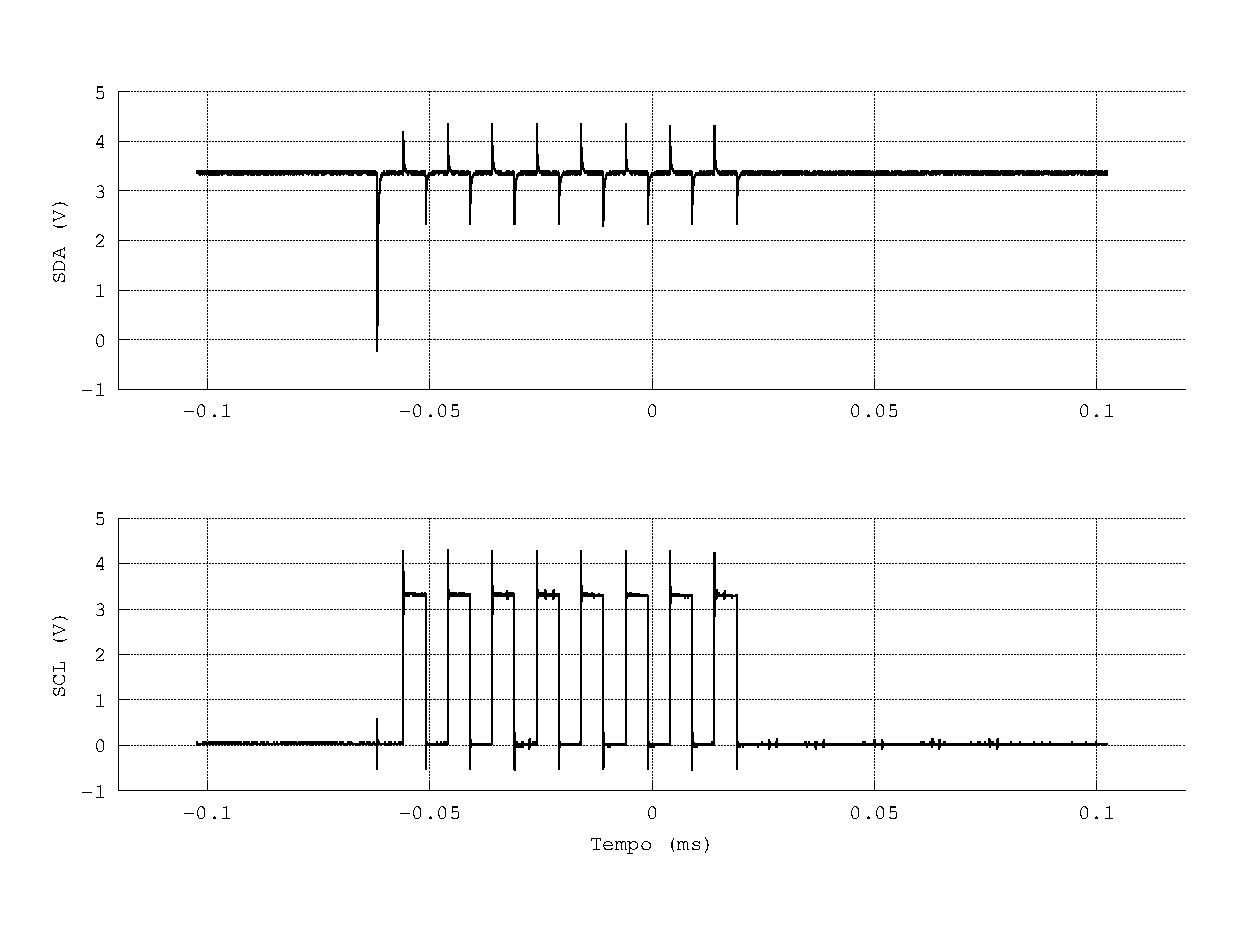
\includegraphics[width=.5\textwidth]{LetturaNero}
	\caption{Fase di lettura: lo \slave{} non scrive niente e il \master{} legge \texttt{0xFF}. Notare i picchi di interferenza dovuti alla capacità $C_C$}
    \label{fig:i2c_lettura}
\end{figure}

\begin{figure}
\centering
  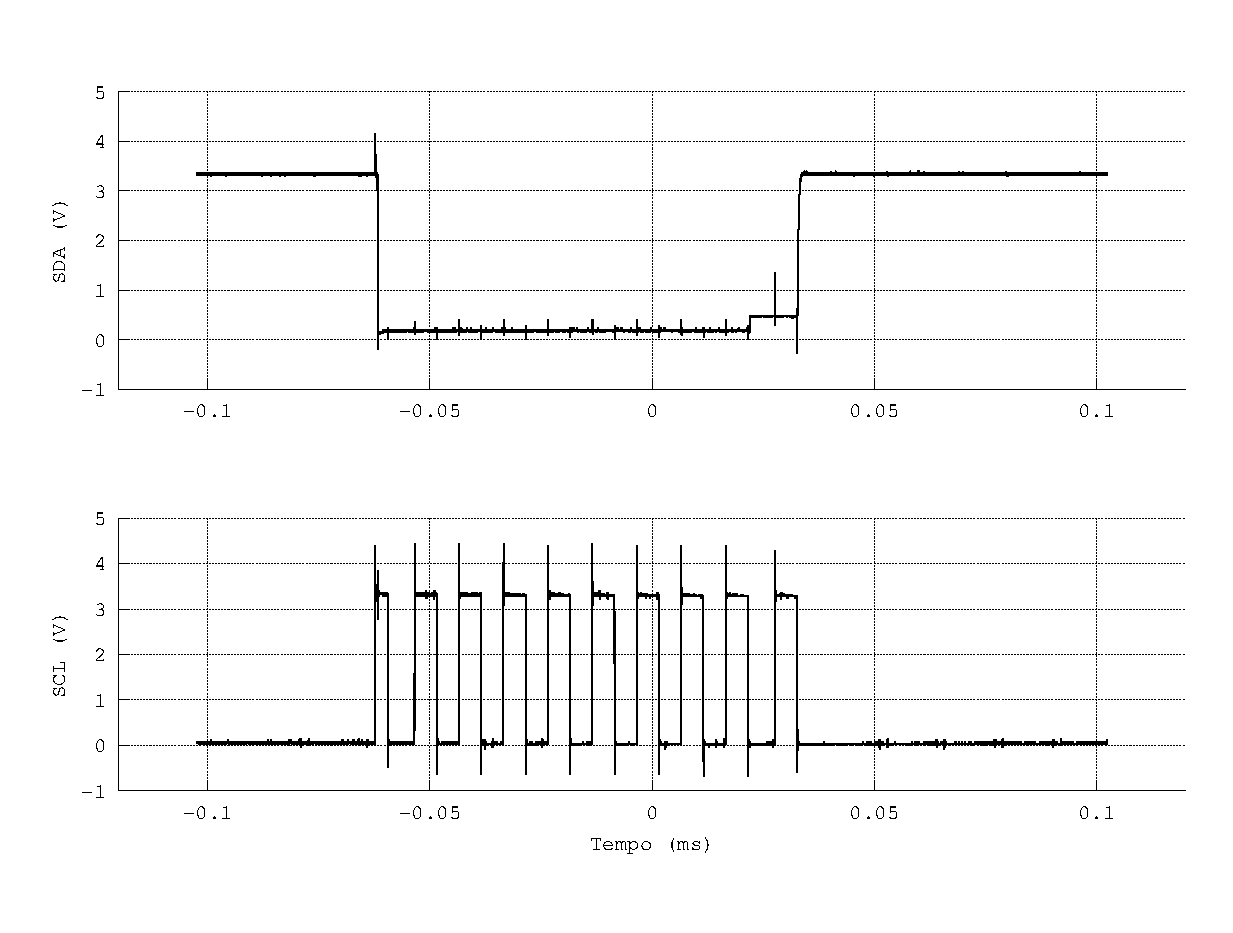
\includegraphics[width=.5\textwidth]{GeneralCallNero}
	\caption{General Call: il \master{} spedisce \texttt{0x00} e lo \slave{} risponde con l'\Ack{}}
    \label{fig:i2c_generalcall}
\end{figure}

\paragraph{Tensione di alimentazione}
	stabile a 3.3V.
    
\paragraph{Tensioni di {\sda} e {\scl}}
	corrette a 3.3 e 0V.

\paragraph{Resistenze di {\pullup}}
Né l'{\relsize{-.5}MSP430} né l'{\relsize{-.5}FT2232H}
sono dotati di opportune resistenze di {\pullup}
o per lo meno non sono configurati per usarle.
Le tensioni che si vedono durante i trasferimenti
sono infatti ottenute dal convertitore {\iic}-{\usb}
\emph{forzando alte} le linee,
cosa che non rispetta il protocollo {\iic}!
Si aggiunge quindi una resistenza da 1k$\Omega$
tra la linea dati e l'alimentazione.

Questa mancanza si manifestava dopo la trasmissione dell'indirizzo,
quando il \master{} (il convertitore {\relsize{-.5}FTDI})
rilasciava la linea dati.
Questa avrebbe dovuto risalire a $V_{CC}$ con la stessa ripidità
dei fronti di salita visti durante la trasmissione,
Si vedeva invece una rampa troppo poco pendente.
La causa di questo è appunto che prima era proprio il \master{}
a tirare su la linea, e il difetto era visibile soltanto
a linea rilasciata. A quel punto si assiste
alla carica della capacità parassita $C_P$
attraverso una resistenza $R_P$ troppo grande,
illustrata in \textsc{Figura~\ref{fig:i2c_rampa}}.\\

\begin{figure}
\centering
  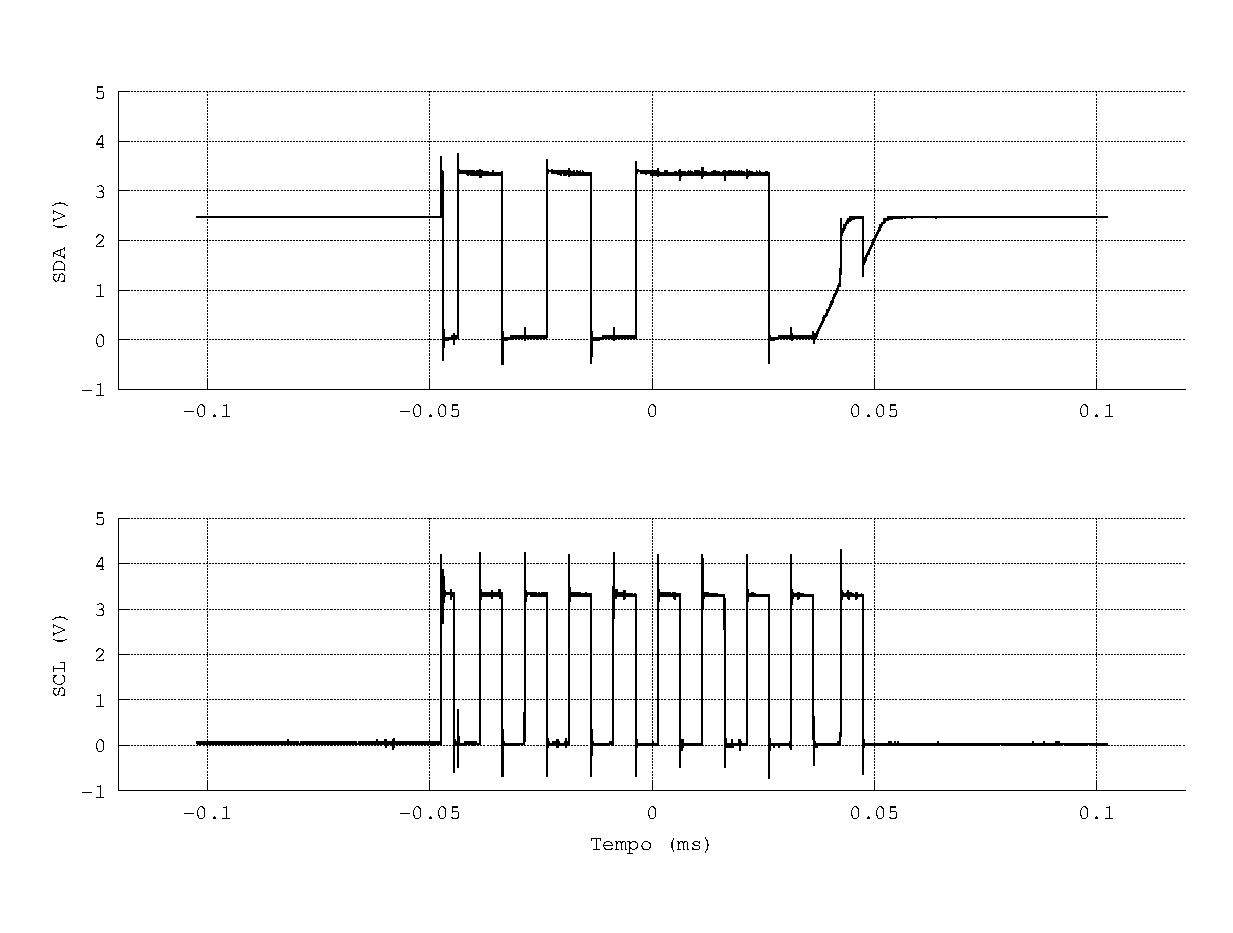
\includegraphics[width=.5\textwidth]{RampaNero}
	\caption{Senza resistenza di \pullup{}: quando il convertitore trasmette, i fronti di salita sono ripidi; quando esso rilascia la linea la tensione sale molto più lentamente.}
    \label{fig:i2c_rampa}
\end{figure}

\paragraph{Picchi di rumore}
In fase di lettura, si notano dei picchi sulla linea dati
in corrispondenza dei fronti del clock.
Questo sarà colpa della capacità parassita
tra le linee $C_C$ di \textsc{Figura~\ref{fig:i2c_tipica}}.\\

\paragraph{Ricapitolando}
Le cause della mancata ricezione degli \Ack{}
e della linea dati sempre alta
riconducono a soglie di tensione non raggiunte o picchi,
che portano all'errata interpretazione dei messaggi
e alla perdita di sincronia.

\subsection{Il convertitore I2C-USB}
%  	Descrizione di quello utilizzato e confronto con gli altri.
    Specifiche richieste:
	\begin{itemize}
	  \item Minimo due canali
	\end{itemize}

    \subsubsection{Due canali} \label{sssez:2canali}
    La specifica deriva dalle osservazioni del paragrafo precedente:
    si è scelto di usare quattro sensori con due soli indirizzi disponibili
    quindi è necessario utilizzare due linee o un \textit{multiplexer}.
    Il modulo di espansione \emph{\relsize{-.5}{FTDI-RPi}} mette a disposizione
    tre porte \usb{} e due canali seriali multiuso
    (a scelta tra \iic{}, {\relsize{-.5} UART} e seriale).
    I produttori forniscono anche le librerie {\relsize{-.5} C++} per l'interfacciamento.
    
	\begin{table}
		% Center the table
		\begin{center}
		% Title of the table
		\caption{Confronto tra i convertitori \iic-\usb}
		\label{tab:convertitori}
		% Table itself: here we have two columns which are centered and have lines to the left, right and in the middle: |c|c|
		\begin{tabular}{r c c}
			% To create a horizontal line, type \hline
%			\hline
			% To end a column type &
			% For a linebreak type \\
Disp.        & Canali (n)  & Prezzo (\euro)\\
			\hline
200XD        &  4          & 8,72\\
USB-ISS      &  1          & 24,89\\
\textbf{Rpi} &  \textbf{2} & \textbf{34,00}\\
			\hline
		\end{tabular}
		\end{center}
	\end{table}

% \input{rpihub.tex}


% {Resta da verificare che questi dispositivi
% non siano sensibili a combinazioni sbagliate di $R_S$ ed $R_P$
% a causa di errate soglie di tensione,
% e sensibili a interferenze e rumore
% a causa della mancanza di Trigger di Schmitt e filtri.}








 \vfill
%% \theendnotes

\chapter{Elaborazione} \label{cap:elab}
		{\bfseries
\vspace{1in}

\paragraph{}
Si vedranno i principali metodi di classificazione.


\paragraph{}
Si introdurranno le machine a vettori di supporto.




\vfill
} \vfill\eject
%	\section{Strumenti utilizzati} \label{sez:strumenti}
%		\subsection{Arduino}
\label{ssez:arduino}







\subsection{MatLab}
\label{ssez:matlab} \vfill
	\section{Algoritmi} \label{sez:algoritmi}
		%% Algoritmi

\subsection{Filtraggio software}
\label{ssez:filtraggio}

Prima di iniziare qualsiasi elaborazione dei dati acquisiti
occorre eseguire delle operazioni di filtraggio,
necessarie a ridurre il rumore e
a diminuire le dimensioni.

Il filtro passabasso per ridurre il rumore è
una media mobile di lunghezza 13;
determinata empiricamente.
Si esegue poi un sottocampionamento di un fattore 5.





\subsection{Classificazione}
\label{ssez:classificazione}

Saranno esposte in seguito i concetti fondamentali
della teoria dei \textit{cluster}
(il termine proposto da \cite{cit:fuzzy} è \textit{botriologia}\footnotemark{}),
e le principali tecniche di classificazione
fino alle macchine a vettori di supporto (\ac{svm}).


\subsubsection{Estrazione delle caratteristiche}
\label{sssez:estrazione}

Al fine di ridurre il più possibile lo sforzo computazionale,
\textbf{aumentando al contempo il significato delle variabili,}
occorre cercare le caratteristiche più rappresentative
dei movimenti in questione.
Tali caratteristiche sono funzione dei movimenti analizzati,
degli esempi proposti e
della classificazione cercata;
possono essere proprietà statistiche come media e varianza,
relazioni più complesse nello spazio e nel tempo
o semplici limitazioni (troppo ampio, troppo lento...).

Queste osservazioni assumono tra l'altro che i dati
siano già in formato vettoriale,
che abbiano quindi la forma di sequenze di numeri
messi in fila o in tabelle di qualsivoglia dimensione.
Se così non fosse, l'estrazione delle caratteristiche
non sarebbe soltanto una comodità per ridurre la mole di calcoli
bensì una necessità per portare gli oggetti in esame
in uno spazio dove queste elaborazioni siano possibili.
Si ritornerà sull'argomento trattando
la mappatura delle \ac{svm}.


\subsubsection{Scelta delle caratteristiche}
\label{sssez:scelta}

Un approccio al problema, tipico della logica sfumata,
\`e conoscere a priori il gesto da valutare e
implementare manualmente le regole di classificazione nel codice della macchina.
Si ottiene così una soluzione specifica.

Quando si vuole invece scoprire queste regole,
occorre avanzare delle ipotesi e poi vagliarle.
Se non si conoscono a priori le caratteristiche significative,
si può procedere estraendone in sovrannumero e
calcolando a posteriori quelle più importanti.
Fatto questo, si possono ``scartare'' le discriminazioni evidenti
e scegliere di concentrarsi sugli aspetti più sottili.
Si preferisce questa soluzione per la sua generalità.






\subsection{Tecniche di classificazione}
Panoramica sulle tecniche statistiche e di apprendimento automatico utili al problema della classificazione.

\subsubsection{K-mean clustering}
Tecnica di classificazione non supervisionata
(non bisogna etichettare i dati prima di far partire l'algoritmo)
che consiste in
\begin{enumerate}
  \item{gettare pi\`u o meno casualmente \emph{K centroidi} nello spazio}
  \item{etichettare ogni punto con l'ID del centroide pi\`u vicino}
  \item{spostare ogni centroide sulla media dei punti a esso assegnati}
  \item{ripetere dal punto 2 finch\'e i centroidi non sono quasi fermi}
\end{enumerate}

\paragraph{Con Matlab}
Il toolbox $statistics$ mette a disposizione il comando $kmeans$ che,
ricevendo in ingresso i punti e il numero di gruppi desiderati,
restituisce le etichette per ogni punto e le coordinate dei centroidi.
Altro scalaggio per visualizzare i dati in 2D.

\paragraph{Crossvalidazione}
Il numero di centri $K$ \`e fissato a priori
ma non sempre si hanno buoni motivi per scegliere un valore pittosto che un altro.
Per trovare il $K$ migliore si fa di solito correre l'algoritmo pi\`u volte,
ogni volta cambiando il $K$ e valutando le prestazioni.
L'insieme dei dati dev'essere preventivamente diviso
in un gruppo di addestramento e un gruppo di test, o validazione.



\subsubsection{Il percettrone classico}
Il percettrone cerca di dividere in due l'universo
mettendoci in mezzo un piano.
Tale piano \`e individuato dai pesi del neurone
e da una soglia, che in pratica \`e un ulteriore sinapsi
con l'ingresso sempre a 1 (o -1, se si preferisce).
La funzione di attivazione può essere la funzione segno, visto che c'è un solo neurone. Se invece si utilizza una rete neurale a più strati con \textit{backpropagation}, occorre adoperare esponenziali o tangenti iperboliche
(\textsc{Equazione~\ref{eq:perceptron}}).

Per ogni vettore d'ingresso
il percettrone calcola 
\begin{equation}
	y = sgn \left(x \cdot w - \theta \right);
	\label{eq:perceptron}
\end{equation}
in fase di addestramento, si confronta l'uscita calcolata
con quella desiderata: $e=d-y$
e si correggono i pesi di un fattore $\Delta w = a\,e\,x$,
dove $a \in [0, 1]$ \`e il fattore di apprendimento.
Analogo per la soglia.

Ad apprendimento concluso i pesi non variano pi\`u
ed il piano di separazione \`e finalmente individuato
dall'equazione \ref{eq:perceptron}, posta uguale a 0.

Una rappresentazione grafica di classificazione eseguita da un percettrone è illustrata in \textsc{Figura~\ref{fig:clus_perc}}

\begin{figure}
\centering
\begin{tikzpicture}

% \draw [red] (-3,-3) grid (3,3);
\draw (-1,1) circle (.25);
\draw (-1,-1) circle (.25);
\draw (-2,-1) circle (.25);
\draw (-2,-2) circle (.25);
\draw (-3,1) circle (.25);

\draw (1,1) ++(-.2,-.2) rectangle ++(.4,.4);
\draw (1,-1) ++(-.2,-.2) rectangle ++(.4,.4);
\draw (2,-1) ++(-.2,-.2) rectangle ++(.4,.4);
\draw (2,-2) ++(-.2,-.2) rectangle ++(.4,.4);
\draw (3,1) ++(-.2,-.2) rectangle ++(.4,.4);

% \node [fill] at (3,3) {};
\draw (-1,-3) -- (1,3)
 node[pos=.7,sloped,above]{iperpiano di separazione};
% % \draw (0,-3) -- (0,3)
% %  node[pos=.8,sloped]{perceptron};


\end{tikzpicture}
\caption{Classificazione con il percettrone}
\label{fig:clus_perc}
\end{figure}

\begin{figure}
\centering
 \begin{tikzpicture}
%
%% Ingresso
  \draw[->](0,0)--(1,0)
    node[pos=.5,above]{\(\bar{x}\)};
%
%% Cornice del neurone
  \draw [dashed, line join=round] (.7,.8) rectangle (5,-.65)
    node [pos=0, above] {Neurone};
%
%% Blocchi del neurone
  \draw (1,-.4)--(2,0)--(1,.4)--cycle;
  \node (w) at (1.3,0) {\(\bar{w}\)};
  \draw[->](2,0)-- ++(.6,0)
    node[pos=.8,above]{\(+\)};
  \draw[<-](2.9,0) ++(-135:.3)--
    ++(-135:.5) node[pos=.2,below]{$-$}
    -- ++(-.6,0)
    node[pos=.5,above]{$\theta$};
  \draw	(2.9,0) node{\(\sum\)} circle (.3);
  \draw[->](3.2,0)-- ++(.6,0);
  \draw (3.8,.4) rectangle ++(.8,-.8);
  \draw (4,-.25)-|(4.2,0)|-(4.4,.25);
%
%% Uscita
  \draw[->](4.6,0)-- ++(1.5,0)
    node[pos=.5,above]{\(y\)};
%
%% Retroazione
  \draw[->](5.5,0)-- ++(0,-.7)
    node[pos=0]{\(\bullet\)}
    node[pos=.8,left]{$-$};
  \draw	(5.5,-1) node{$\sum$} circle (.3);
  \draw[<-](5.8,-1)-- ++(.6,0)
    node[pos=0.2,below]{$+$}
    node[pos=0.6,below]{$d$};
  \draw[<-](1.3,-.3) |- (2.5,-1)
    node[pos=.5,,below]{\(\Delta w_i = a\,e\,x_i\)};
  \draw (3.3,-.7)--(2.5,-1)--(3.3,-1.3)--cycle;
  \node (a) at (3.03,-1) {$a$};
  \draw[<-](3.3,-1)--(5.2,-1)
    node[pos=.5,below]{$e$};
    
\end{tikzpicture}

 \caption{Schema a blocchi del percettrone}
 \label{fig:perceprton}
\end{figure}

\subsubsection{L'apprendimento competitivo}
Apparentemente simile al K~-~means,
\`e l'apprendimento competitivo\footnotemark{}.

\footnotetext{\,Non sono la stessa cosa e non portano agli stessi risultati}

Consiste nello strutturare una rete di $K$ neuroni
ciascuno con il suo vettore dei pesi
inizialmente casuale ma sempre di modulo 1.
In questo modo a ogni neurone \`e assegnato un versore
in un qualche spazio.
I neuroni sono tra loro collegati tramite linee di segnali inibitori.
Quando le coordinate di un punto di addestramento
sono date in pasto alla rete,
ci sar\`a un neurone che indica in quella direzione,
o per lo meno un neurone sar\`a pi\`u vicino degli altri:
questo \`e l'unico neurone autorizzato ad apprendere
e modificher\`a i suoi pesi in maniera da avvicinarsi
un po' alla direzione del punto.
L'apprendimento degli altri neuroni \`e inibito.

Questa tecnica richiede ulteriori pretrattamenti dei dati in ingresso
in maniera che siano distribuiti (meglio possibile)
su una sfera centrata nell'origine. \vfill
	\section{Macchine a vettori di supporto} \label{sez:svm}
		Si attribuisce a Vapnik l'applicazione fruttuosa
del kernel all'apprendimento automatico (1992).

\subsection{Il Kernel}
Prende il nome da qualche teoria matematica avanzata.
Per capirsi
\subparagraph{Il prodotto scalare \`e un kernel} Presi due vettori, due elementi di uno spazio
in cui sia definito un prodotto scalare,
il kernel sar\`a un'estensione del prodotto scalare consueto
\subparagraph{Il kernel \`e un prodotto scalare} L'idea è
di portarsi in un comodo spazio dotato di prodotto scalare
per poi applicare il kernel


Formalmente:
\begin {equation}
  \label {eq:kernel}
  k = \langle \mathbf{\Phi}(x_1), \mathbf{\Phi}(x_2) \rangle
\end{equation}
dove $\mathbf{\Phi}(x)$ \`e una mappa -se si vuole- non lineare
che porta i generici elementi $x$
in uno spazio dotato di prodotto scalare.

NB$_{1}$: Gli elementi originali possono quindi non essere neanche vettori.\par
NB$_{2}$: In generale \`e pi\`u semplice scrivere la funzione kernel piuttosto che la mappa.\par
Oss: Praticamente si stanno estraendo le caratteristiche.\par

\subsubsection{Il kernel e l'apprendimento automatico}
Rimanendo nell'ambito della classificazione binaria
la funzione discriminante \`e
\begin{equation}
	\label{eq:discriminante}
	y_n = sgn \left(\langle w, \mathbf{\Phi}(x_n) \rangle + b \right)
\end{equation}
ma si definiscono i pesi come
\begin{equation}
  \label{eq:pesikernel}
  w = \sum_i y_i \alpha_i \mathbf{\Phi}(x_i)
\end{equation}
con $\alpha_i$ che \textbf{come si chiama?}
Sostituendo la \ref{eq:pesikernel} nella \ref{eq:discriminante}
si ottiene
\begin{align}
  y_n &= sgn \left(\sum_i y_i \alpha_i \langle \mathbf{\mathbf{\phi}}_i,\mathbf{\mathbf{\phi}}_n \rangle + b \right) \\
  &= sgn \left(\sum_i y_i \alpha_i k(x_i,x_n) + b \right)
  \label{eq:uscitakernel}
\end{align}

\subsubsection {Il kernel perceptron}
(Tratto da un articolo dell'Universit\`a di Trento).
L'algoritmo di apprendimento \`e molto simile
a quello del percettrone classico.
La differenza sta nel calcolo della funzione (vedi eq. precedente)
e nell'aggiornamento dei pesi:
gli $\alpha_i$ sono incrementati ogni volta che
il neurone sbaglia la previsione su un $x_i$.


\subsubsection {\acf{spra}}
Schoelkopf e Smola propongono un semplice algoritmo di classificazione
introduttivo alle macchine a vettori di supporto (\ac{svm}).

Non si fa altro che prendere i punti medi delle due classi ($c_1$ e $c_2$),
prendere il vettore differenza trai due $w=c_1-c_2$
il loro punto medio ($c=(c1+c2)/2$).

Ora ogni altro punto di classe ignota
pu\`o essere etichettato con
\(y =sgn \left( \langle \boldsymbol{x-c}, \boldsymbol{w} \rangle \right)\).



\subsection {\acf{svm}}
Sono algoritmi che usano l'espediente del kernel
per mappare le sequenze in degli spazi comodi
(tipicamente con molte dimensioni in pi\`u)
dove trovare il piano di separazione che massimizza il margine (\textsc{Figura~\ref{fig:clus_svm}}).
Nello spazio di partenza la separazione pu\`o assumere le forme pi\`u diverse
(dipende dalla mappa non lineare).

Il problema \`e posto nei termini di minimizzazione della lagrangiana
\begin{equation}
    L_P = lagrangiana
  \label{eq:lagrangiana}
\end{equation}
o massimizzazione della sua duale
\begin{align}
  \label{eq:lagr_duale}
  L_D &= \sum_i \alpha_i - \frac{1}{2} \sum_i \sum_j \alpha_i \,\alpha_j \,y_i \,y_j \,k(\boldsymbol{x_i}, \boldsymbol{x_j}) \\
  \langle \boldsymbol{\alpha}, \boldsymbol{y} \rangle &= 0 \\
  \alpha_i &\geq 0
\end{align}

\begin{figure}
\centering
\begin{tikzpicture}

% \draw (-8, -5) grid (5, 5);

\draw [fill] (-1,1) circle (.25);
\draw [fill] (-1,-1) circle (.25);
\draw (-2,-1) circle (.25);
\draw (-2,-2) circle (.25);
\draw (-3,1) circle (.25);

\draw [fill] (1,1) ++(-.2,-.2) rectangle ++(.4,.4);
\draw [fill] (1,-1) ++(-.2,-.2) rectangle ++(.4,.4);
\draw (2,-1) ++(-.2,-.2) rectangle ++(.4,.4);
\draw (2,-2) ++(-.2,-.2) rectangle ++(.4,.4);
\draw (3,1) ++(-.2,-.2) rectangle ++(.4,.4);

\draw [dashed] (-1,-3) -- (1,3)
 node[pos=.9,sloped,above]{perceptron};
\draw (0,-3) -- (0,3)
 node[pos=.9,sloped,above]{\acs{svm}};

% \draw (-5,-2) circle (.125);
% \draw (-5,-1) circle (.125);
% \draw (-6,-1) circle (.125);
% \draw (-6,-2) circle (.125);
% \draw (-7,-2) circle (.125);

% \draw (-6.5,-1.3) ++(-.1,-.1) rectangle ++(.2,.2);
% \draw (-6,0) ++(-.1,-.1) rectangle ++(.2,.2);
% \draw (-6.7,-3) ++(-.1,-.1) rectangle ++(.2,.2);
% \draw (-5.5,-3.4) ++(-.1,-.1) rectangle ++(.2,.2);
% \draw (-4.7,-2.1) ++(-.1,-.1) rectangle ++(.2,.2);

% \draw [->, ultra thick] (-4.5, -2.5) -- (-2, 0)
%   node [pos=.5, sloped, above] {mappa $\Phi$};

\end{tikzpicture}
\caption{L'\acs{svm} trova il piano di separazione che massimizza il margine}
\label{fig:clus_svm}
\end{figure}

\subsubsection{Ottimizzazione con MatLab}
Per eseguire lquesta operazione si utilizza la funzione
\(fmincon\) di ottimizzazione vincolata.

\par
Questa strumento prende in ingresso
la funzione obiettivo e la funzione supporto,
vale a dire la funzione da minimizzare e i vincoli non lineari da rispettare;
il punto di partenza;
gli eventuali vincoli lineari di uguaglianza e disuguaglianza.


 \vfill

%% \theendnotes

\chapter{Verifica sperimentale} \label{cap:verifica}
		{\bfseries
\vspace{1in}

\paragraph{}
sommario

\vfill
} \vfill\eject
 \section{Impostazione teorica}
%	\subsection{Cosa si vuole verificare} \label{sez:cosa}
		Si vuole verificare l'applicabilit\`a delle macchine a vettori di supporto alla valutazione dei gesti motori.

 \vfill
%	\subsection{Criteri di valutazione} \label{sez:criteri}
		Si prova innanzitutto la macchina sull'insieme di dati \emph{Iris},
tipicamente utilizzato per testare i classificatori.

Ne risulta un tasso di successo anche del 100\% (\textsc{Figura~\ref{fig:iris100}}).

\begin{figure}
  \centering
  \resizebox{.9\textwidth}{!}{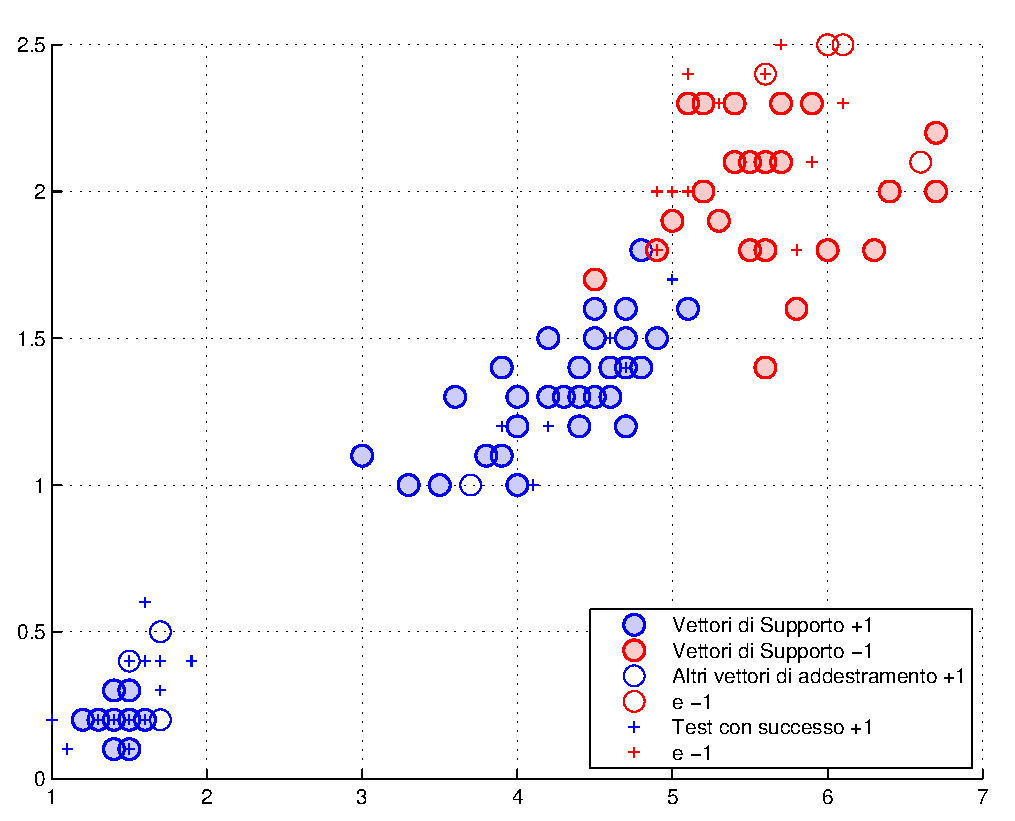
\includegraphics{Disegni/Iris100}}
  \caption{La \ac{svm} testata sul \textit{Iris} ottiene un tasso di successo fino al 100\%.}
  \label{fig:iris100}
\end{figure}

La si addestra poi seguendo i protocolli proposti in letteratura
e lo si collauda su un insieme di test.

Le risposte fornite dalla macchina sono confrontate con i giudizi dell'esperta. \vfill
		\subsection{Esperimenti possibili}
\label{ssez:esp_possibili}



\subsection{Esperimenti fattibili}
\label{ssez:esp_fattibili}



\subsection{Impostazione di un esperimento}
\label{ssez:impost_esp} \vfill
	\section{Realizzazione di un esperimento} \label{sez:esperimento}
		Si propone un'esperimento con un gesto più complesso
di quelli visti nella \textsc{Sezione~\ref{sez:biomeccanica}},
il \textit{Port de bras} della danza classica.

\subsection{Descrizione del movimento}
I motivi per cui è stato scelto questo gesto sono  
\begin{itemize}
	\item coinvolge soltanto un arto, lasciando fermo il resto del corpo monte della spalla
    \item è abbastanza lento da poter essere rilevato con tutti gli accelerometri disponibili, sia rispetto al campo di misura, che alla frequenza di campionamento
    \item è semplice dal punto di vista cinematico
    \item è altrettanto facile da sbagliare
\end{itemize}

\paragraph{Fasi del movimento}
\begin{enumerate}
	\item \textbf{Posizione di partenza:} con il braccio rotondo e la spalla giù, portare la mano 5cm in avanti rispetto alla posizione di riposo
    \item \textbf{Elevazione:} tenendo la spalla bassa e il gomito sostenuto, alzare la mano fino all'altezza dell'ombelico
    \item \textbf{Apertura:} aprire il braccio, sempre rotondo \emph{non} al di fuori del campo visivo e \emph{non} dietro alla spalla.
\end{enumerate}

\paragraph{Ulteriori precisazioni e possibili errori}
\begin{itemize}
    \item [$\checkmark$] attenzione a mantenere il braccio ovale
    \item [$\checkmark$] alzare all'altezza dell'ombelico, non del volto
    \item [$\checkmark$] prima si sale e \emph{poi} si apre, non tutto insieme
	\item[$\times$] mano decentrata
   	\item[$\times$] gomito disteso
	\item[$\times$] alla fine, gomito troppo basso rispetto alla spalla
   	\item[$\times$] mano troppo indietro
\end{itemize}






\subsection{Fase di acquisizione e raccolta dei dati}

\paragraph{Strumenti e persone} 

\begin{itemize}
  \item accelerometro e applicazione per la raccolta dei dati a bordo di un telefono cellulare
  \item telecamera
  \item una persona esperta
  \item due persone non esperte.
\end{itemize}
Nota bene: tutti gli interessati sono destrimani.

\paragraph{Preparazione}
D'accordo con l'esperta,
si è deciso di raccogliere un numero di esempi
simile a quello che si avrebbe all'inizio di una seduta di allenamento,
con l'istruttrice che per la prima volta spiega l'esercizio agli allievi:
\begin{itemize}
	\item[10] esempi corretti della maestra
    \item[10$\times$2] esempi degli allievi da valutare (verosimilmente scorretti) 
    \item[2$\times$Err] esempi scorretti della maestra
    \item[5] altri esempi corretti della maestra
    \item[10$\times$2] esempi degli allievi da valutare (verosimilmente migliori di prima)
    \item[5$\times$2] movimenti intenzionalmente scorretti e rumorosi
\end{itemize}
A turno gli esecutori prendono lo \textit{smartphone} e
si posizionano in modo da non avere ostacoli che impediscano i movimenti
ed avere una buona luce per le riprese.
Si cerca di far partire contemporaneamente registrazione e riprese.
Gli esempi sono registrati sulla stessa traccia.
Si pone un'attesa di circa due secondi prima del gesto,
una di tre secondi alla fine, col braccio ancora alto),
poi si riabbassa il braccio e,
una volta in posizione di partenza,
si attendono di nuovo i due secondi e si ripete.



\subsubsection{Estrazione degli esempi dalle tracce}
Gli esempi raccolti nella fase precedente vengono estratti dalle registrazioni,
che ne contengono da cinque a dieci.

Come scritto nel paragrafo precedente,
si acquisiscono cinque, dieci esempi per traccia
che devono essere poi estratti.

A seconda della complessità del movimento e
della facilità con cui si possono riconoscere i \textit{pattern} nelle tracce,
l'estrazione può essere più o meno automatizzata.
Nel caso in questione, si è preferito \textbf{prendere} i \textit{timestamp}
dalle riprese video e \textbf{ritagliare} quindi i segmenti in MatLab.
Ogni esempio ha un suo tempo di esecuzione e
conseguentemente un diverso numero di campioni,
quindi si è deciso di uniformarne la durata a cinque secondi
(equivalenti a cento campioni),
e \textbf{porre gli altri campioni costanti}.

Prima di questa fase è consigliabile filtrare le tracce con un passabasso per ridurre il rumore,
poi ridurre la frequenza di campionamento (\textsc{Sottosezione~\ref{ssez:filtraggio}}).
\subsection{Fase di Elaborazione}

{\bfseries Considerazione sulla fase di elaborazione,
come ad esempio la crossvalidazione su $C$}

% \subsubsection{Risultati dell'esperimento} \vfill
%% \theendnotes



\chapter{Conclusioni} \label{cap:conclusioni}
		{\bfseries

\paragraph{}
Si traggono in questo capitolo le conclusioni sul sistema sviluppato e sul lavoro in generale.

\paragraph{}
Si suggeriscono infine gli ulteriori miglioramenti e applicazioni possibili.
} \vfill\eject
	\section{Conclusioni} \label{sez:risultati}
		La discreta percentuale di successi ottenuta nell'esperimento
non lascia escludere di poter valutare gesti motori anche complessi
con un solo accelerometro, anche di fascia bassa.

Il classificatore realizzato si dimostra eccessivamente \emph{severo},
giudicando come $sbagliati$ anche due esempi della maestra.
Questo comportamento potrebbe tuttavia essere causato da imperfezioni
nell'esecuzione e non da un errore di classificazione.

Per le considerazioni fatte nella \textsc{Sottosezione~\ref{rif:problema}}
è comunque preferibile che il sistema dia falsi negativi --come in effetti fa,
piuttosto che falsi positivi.

I risultati sono incoraggianti 
seppure il numero di esempi non sia statisticamente significativo. \vfill
	\section{Sviluppi futuri} \label{sez:sviluppi}
		\begin{itemize}
	\item Trasmissione senza fili
    \item Aumentare gli esempi
    \begin{itemize}
		\item mantenendo le percentuali tra esempi di esperti e non
    	\item anche provenienti da piattaforme hardware diverse
	\end{itemize}
    \item Aumentare i sensori
    \begin{itemize}
		\item per tracciare la catena cinematica completa
    	\item per fornire la diagnostica
	\end{itemize}
    \item eseguire su microcontrollore o \textit{smartphone}
\end{itemize}
 \vfill
%% \theendnotes






%%%%%%%%%%%%%%%%%%%%%%%%%%%%%%%%%%%
%%%%%%%%%%%%%%%%%%%%%%%%%%%%%%%%%%%
%%%%%%%%%%%%%%%%%%%%%%%%%%%%%%%%%%%

\eject
\newpage
\thispagestyle{empty}
\mbox{}

\appendix{}
%\input{Capitoli/App/Dimensioni}

\eject
\newpage
\thispagestyle{empty}
\mbox{}

\listoffigures
\begingroup
\let \clearpage \relax
\addcontentsline{toc}{chapter}{Elenco delle figure, delle tabelle e dei codici}
\vfill \listoftables
\vfill \lstlistoflistings
\endgroup
%\addcontentsline{toc}{section}{\listfigurename}
%\addcontentsline{toc}{section}{\listtablename}
%\addcontentsline{toc}{section}{\lstlistlistingname}
\eject
\newpage
\thispagestyle{empty}
\mbox{}

%\include{Bibliografia}
\bibliographystyle{natbib_ita}
\bibliography{bib}
\addcontentsline{toc}{chapter}{\refname}
\vfill\eject

\newpage
\thispagestyle{empty}
\mbox{}
\chapter{Ringraziamenti}

\end{document}